\documentclass[12pt,a4paper,fontset=none]{ctexart}
\usepackage[margin=2.2cm]{geometry}
\usepackage{array}
\usepackage{booktabs}
\usepackage{longtable}
\usepackage{graphicx}
\usepackage{float}
\usepackage{multirow}
\usepackage{enumitem}
\usepackage{hyperref}
\usepackage{titlesec}
\usepackage{caption}

\setmainfont{Times New Roman}
\setsansfont{Arial}
\setmonofont{Menlo}
\setCJKmainfont{Songti SC}
\setCJKsansfont{Heiti SC}
\setCJKmonofont{STSong}

\titleformat{\section}{\bfseries\Large}{\thesection}{0.8em}{}
\titleformat{\subsection}{\bfseries\large}{\thesubsection}{0.8em}{}
\setlist[itemize]{nosep}
\setlist[enumerate]{nosep}
\captionsetup{font=small}
\newcommand{\phitol}[3]{\ensuremath{\Phi #1^{#2}_{#3}}}

\begin{document}

    \begin{titlepage}
        \centering
        \vspace*{2.5cm}
        {\zihao{2}\bfseries 2026年春季学期《机械制造技术基础》课程大作业中批量机械加工831009(CA6140车床杠杆)零件的关键工艺问题分析\par}
        \vspace{1.2cm}

        \zihao{4}
        班号：\underline{\hspace{6cm}}\par
        \vspace{0.3cm}
        学号：\underline{\hspace{6cm}}\par
        \vspace{0.3cm}
        姓名：（签字）\underline{\hspace{6cm}}\par
        \vspace{0.3cm}
        同组同学姓名：\underline{\hspace{6cm}}\par
        \vspace{0.3cm}
        评阅教师：\underline{\hspace{6cm}}\par
        \vspace{0.3cm}
        评阅成绩：\underline{\hspace{6cm}}\par
        \vspace{0.3cm}
        评阅日期：\underline{\hspace{6cm}}\par

        \vfill
    \end{titlepage}

    \tableofcontents
    \newpage


    \section{零件图分析}

    \subsection{零件作用简介}

    该零件为CA6140普通车床主轴箱操纵机构的杠杆，是典型的摇臂式传力构件，材料为HT200灰铸铁，核心作用与特点如下：

    \begin{enumerate}
        \item \textbf{核心功能：}作为车床变速系统的中间传动件，以中心$\phi22.5$孔为回转支点，将操纵手柄的手动运动与力传递给拨叉机构，推动主轴箱内的滑移齿轮完成啮合切换，从而实现主轴转速的调节或换向控制，是车床手动控制链中不可或缺的关键零件。
        \item \textbf{工况与结构特点：}
    \end{enumerate}

    \begin{itemize}
        \item \textbf{受力复杂：}承受双向交变载荷，中心孔与操纵轴的配合精度直接决定操纵手感的顺滑度与机构的长期可靠性。
        \item \textbf{多工作面集成：}包含中心安装孔、连接螺纹孔、定位销孔及多组安装定位面，需同时满足传动、连接、定位三类功能，结构呈多叉臂的空间分布。
        \item \textbf{铸造工艺性：}采用灰铸铁铸造，兼具良好的减震性、耐磨性与铸造工艺性，适合批量生产复杂结构零件。
    \end{itemize}

    \subsection{零件图改进}

    针对图中视图表达、尺寸标注、工艺标注等问题，进行系统性改进，具体如下表所示：

    \begin{table}[H]
        \centering
        \caption{零件图改进}
        \label{tab:drawing_fix}
        \begin{tabular}{p{1.2cm} p{2.2cm} p{3.2cm} p{3.8cm} p{3cm} p{1cm} }
            \toprule
            序号 & 改进类别    & 错误点                                & 改进方案                                 & 图示 \\
            \midrule
            1  & 视图表达改进  & 左视图（左侧视图）投影错误，线型使用混乱               & 按“长对正、高平齐、宽相等”修正轮廓线，保证与主视图槽口、孔系的投影对应 & 略  \\
            2  & 尺寸标注改进  & 尺寸标注位置混乱、交叉                        & 将交叉的尺寸线调整至视图外部                       & 略  \\
            3  & 结构改进    & 零件上方两个螺栓孔未标注尺寸且其中一孔未倒角             & 标注尺寸，对未倒角孔进行 120°倒角，轴向尺寸为2 mm        &
            \begin{minipage}[b]{0.22\columnwidth}
                \centering
                {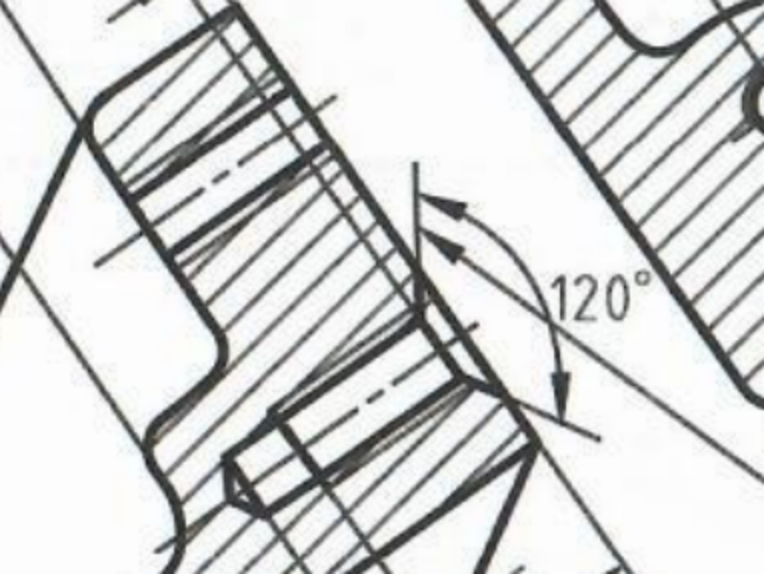
\includegraphics[width=0.9\textwidth]{Img/图片3.png}}
            \end{minipage} \\

            4  & 表面粗糙度改进 & 左侧视图外轮廓面缺少粗糙度标注                    & 按国标绘制完整粗糙度符号，尖角指向材料表面。                &
            \begin{minipage}[b]{0.9\linewidth}
                \centering
                \raisebox{-0.5\height}{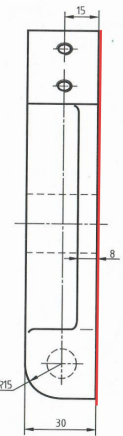
\includegraphics[width=0.9\linewidth]{Img/图片4.png}}
            \end{minipage} \\
            5  & 表面粗糙度改进 & M8螺栓支承面Ra1.6的粗糙度过低                 & 将该面粗糙度修正为Ra3.2，与普通螺栓支承面的通用要求匹配，节约成本。  &
            \begin{minipage}[b]{0.9\linewidth}
                \centering
                \raisebox{-0.5\height}{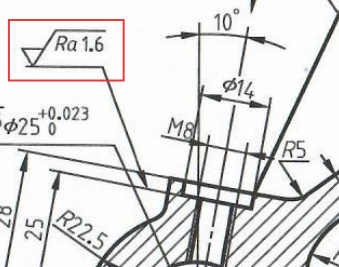
\includegraphics[width=0.9\linewidth]{Img/图片5.png}}
            \end{minipage} \\
            6  & 结构工艺性改进 & 左侧视图阶梯过渡转角为直角，未标注铸造圆角，易产生铸造缺陷与应力集中 & 在该转角处添加 R3~R5 的铸造圆角，按国标绘制圆角轮廓线       &
            \begin{minipage}[b]{0.9\linewidth}
                \centering
                \raisebox{-0.5\height}{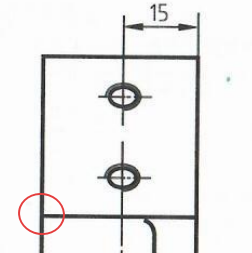
\includegraphics[width=0.9\linewidth]{Img/图片6.png}}
            \end{minipage} \\

            \bottomrule
        \end{tabular}
    \end{table}

    \subsection{机械加工过程的关键工艺问题}

    \subsubsection{关键孔系的位置精度与尺寸精度控制}

    \begin{enumerate}
        \item \textbf{中心孔$\phi22.5$H7的加工：}该孔是杠杆的回转支点，需与操纵轴形成间隙配合，孔的圆度、圆柱度及表面粗糙度（Ra1.6）直接影响操纵手感与磨损寿命。

        \textbf{加工难点：}孔的精度要求高，需采用“粗镗$\rightarrow$半精镗$\rightarrow$铰孔”的工艺路线，同时保证孔轴线与两臂的角度定位精度，加工时易因装夹误差导致位置超差。
        \item \textbf{$\phi12.7$定位销孔与M8螺纹孔的位置度控制：}两孔与中心孔的中心距、角度公差直接影响杠杆与拨叉的装配精度，需保证孔系的位置度误差$\leq 0.1$mm。

        \textbf{加工难点：}$\phi12.7$孔需用钢球检查，对孔的同轴度与位置度要求高，加工时易因钻头偏斜导致孔口椭圆度误差；M8螺纹孔需控制攻丝深度，避免过切或螺纹有效长度不足。
    \end{enumerate}

    \subsubsection{多工位装夹与基准统一问题}

    \begin{enumerate}
        \item \textbf{多次装夹的基准不重合误差：}杠杆为多叉臂结构，加工不同工作面时需多次装夹，易产生基准不重合误差，导致各工作面的位置精度超差。

        \textbf{解决思路：}设计专用夹具，以$\phi22.5$中心孔和铸造基准面为统一基准，实现一次装夹完成多面加工，减少装夹次数。
        \item \textbf{铸造毛坯的工艺余量控制：}铸件拔模斜度、铸造圆角易导致毛坯余量不均，粗加工时易出现局部余量不足或刀具振动。

        \textbf{解决思路：}粗加工前对毛坯进行划线找正，合理分配粗加工余量，选择硬质合金刀具，优化切削参数，减少刀具磨损。
    \end{enumerate}

    \subsubsection{表面质量与工艺性优化}

    \begin{enumerate}
        \item \textbf{关键工作面的表面粗糙度控制：}中心孔、安装面的Ra1.6$\sim$Ra3.2要求较高，精加工时易因积屑瘤、刀具磨损影响表面质量，需控制切削速度与进给量，采用合适的冷却润滑方式。
        \item \textbf{铸造缺陷的预处理：}毛坯表面易存在气孔、砂眼，加工前需进行时效处理消除内应力，粗加工后对缺陷进行焊补或打磨，避免影响后续加工与零件强度。
    \end{enumerate}

    \begin{figure}[H]
        \centering
        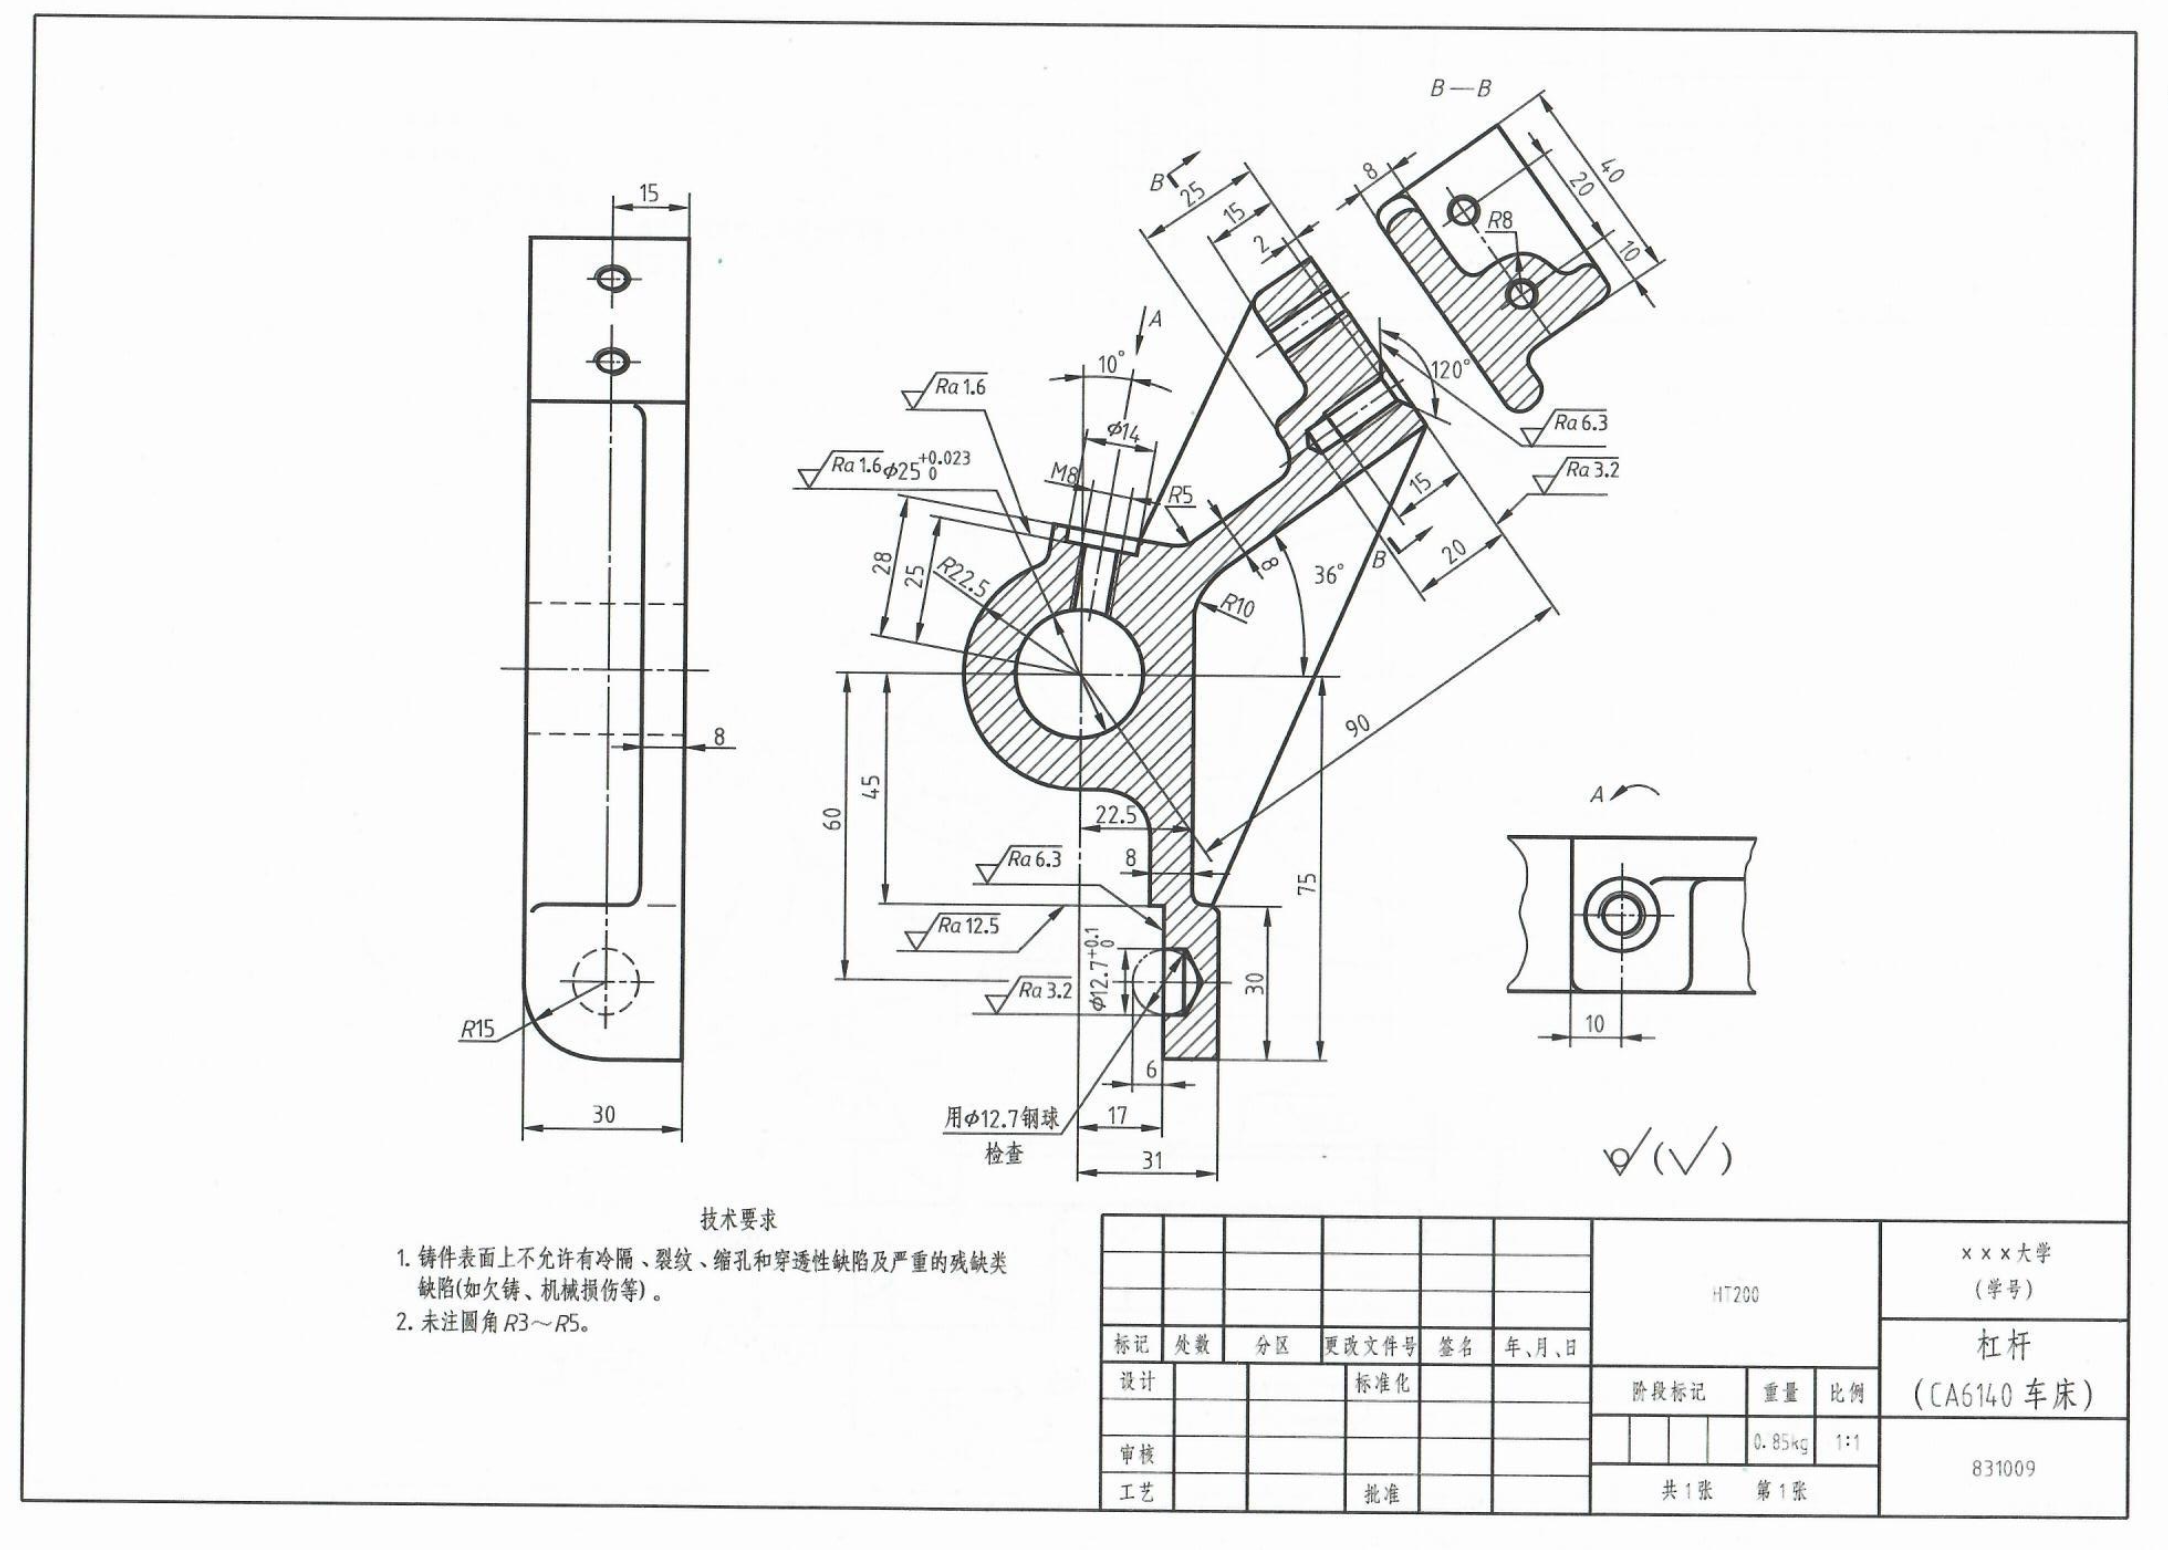
\includegraphics[width=0.92\textwidth]{杠杆（CA6140车床）831009.png}
        \caption{杠杆零件工作图}
    \end{figure}


    \section{工艺路线设计}

    \subsection{机械加工工艺分析}

    \subsubsection{毛坯选择}

    零件CA6140车床杠杆的材料为HT200，而且零件的轮廓尺寸不大，铸造表面质量的要求高，故可采用铸造质量稳定的，适合大批生产的金属模铸造，又考虑到本零件在具体工作的受力情况，也可以选择砂型铸造，足以满足要求。最终选择金属模铸造，其便于铸造和加工工艺过程，而且还可以提高生产率。

    根据灰口铸铁HT200的密度以及给定的零件图计算出毛坯质量约为1kg，生产类型属于轻型零件。

    \subsubsection{主要加工表面}

    零件的材料为HT200，灰铸铁生产工艺简单，铸造性能优良，但塑性较差、脆性高，为此以下是杠杆需要加工表面以及加工表面的位置要求。现分析如下：

    \paragraph{主要加工面}

    \begin{itemize}
        \item \textbf{小头孔及相邻孔系：}小头钻\phitol{25}{+0.023}{0}以及与此孔相通的$\Phi14$阶梯孔、M8螺纹孔。
        \item \textbf{锥孔及平台：}钻\phitol{12.7}{+0.1}{0}锥孔及铣\phitol{12.7}{+0.1}{0}锥孔平台。
        \item \textbf{螺纹孔：}钻2−M6螺纹孔。
        \item \textbf{平面：}铣杠杆底面及2−M6螺纹孔端面。
    \end{itemize}

    \paragraph{主要基准面}

    \begin{itemize}
        \item \textbf{以$\Phi45$外圆面为基准的加工表面：}这一组加工表面包括\phitol{25}{+0.023}{0}的孔、杠杆下表面。
        \item \textbf{以\phitol{25}{+0.023}{0}的孔为中心的加工表面：}这一组加工表面包括$\Phi14$阶梯孔、M8螺纹孔、\phitol{12.7}{+0.1}{0}锥孔及$\Phi$锥孔平台、2−M6螺纹孔及其倒角。其中主要加工面是M8螺纹孔和\phitol{12.7}{+0.1}{0}锥孔平台。
    \end{itemize}

    \subsubsection{机械加工余量与加工阶段划分}

    根据以上毛坯选择分析及加工工艺分析，即杠杆的材料是HT200，毛坯的重量约1kg，生产类型为大批生产，毛坯采用金属模铸造, 根据铣刀类型及尺寸、毛坯及零件情况可知选用6mm的铣刀进行粗加工,半精铣与精铣的加工余量都为0.5mm。分别对个加工表面的确定如下：

    \begin{enumerate}
        \item \textbf{零件底面：}此面是粗基准，是最先加工的表面。由《机械加工工艺设计实用手册》表6-92及公式（6-16）e = C 计算底面加工余量为e=2.5mm。
        \item \textbf{加工$\Phi25$的端面：}根据参考文献[1]表4-35和表4-37考虑以及查表可得3mm，粗加工2mm到金属模铸造的质量和表面的粗糙度要求，精加工1mm，同理上下端面的加工余量都是e=2mm。
        \item \textbf{对$\Phi25$的内表面加工：}由于内表面有粗糙度要求1.6。可用一次粗加工1.9mm，一次精加工0.1mm就可达到要求。

        中间孔（$\Phi25$）：毛坯为实心，不冲出孔，孔精度为IT7—IT8之间。
        根据《机械加工工艺设计实用手册》确定步骤为：

        钻孔：$\Phi23$；

        扩孔：$\Phi24.8$，余量 e = 1.8mm；

        粗铰：$\Phi24.94$，余量 e = 0.14mm；

        精铰：$\Phi25$，余量 e = 0.06mm。
        \item \textbf{加工宽度为30mm的下平台：}用铣削的方法加工台肩。由于台肩的加工表面有粗糙度的要求$R_a=6.3um$，而铣削的精度可以满足，故采取分四次的铣削的方式，每次铣削的深度是2.5mm。
        \item \textbf{钻锥孔$\Phi12.7$：}要求加工一半，留下的余量装配时钻铰，为提高生产率起见，仍然采用$\Phi12$的钻头，切削深度是2.5mm。
        \item \textbf{钻Ф14阶梯孔：}由于粗糙度要求$R_a=6.3um$，因此考虑加工余量2mm。可一次粗加工1.85mm，一次精加工0.15mm就可达到要求。
        \item \textbf{加工M8底孔：}根据参考文献[1]表4-23考虑加工余量1.3mm。可一次钻削加工余量1.1mm，一次攻螺纹0.1mm就可达到要求。

        M8螺纹孔：毛坯为实心。根据《机械制造工艺手册》，M8底孔为6.7。具体如下：钻M8底孔$\Phi6.7$； 攻丝M8，余量 e = 1.3mm。
        \item \textbf{加工2−M6螺纹：}根据参考文献[1]表4-23考虑加工余量0.8mm。可一次钻削加工余量1.1mm，一次攻螺纹0.1mm就可达到要求。

        M6螺纹孔：毛坯为实心。根据《机械制造工艺手册》，M6底孔为5.2。具体如下：
        钻M6底孔$\Phi5.2$；
        倒角120°；
        攻丝M6，余量 e = 0.8mm。
        \item \textbf{加工2−M6端面：}粗加工2mm到金属模铸造的质量和表面粗糙度要求，精加工1mm，可达到要求。
    \end{enumerate}

    \subsection{工艺基准的选择}

    基准面的选择是工艺规程设计的重要过程之一。基面的选择正确与否，可以是加工质量的到保证，生产效率提高，否则，不但加工工艺过程漏洞百出，更有甚者，零件的大批量的报废，使用无法进行，难以在工期内完成加工任务。

    \subsubsection{设计基准分析}

    从零件的使用要求看，中心孔轴线是零件最核心的设计基准，零件上的多个孔、端面和工作臂位置关系均围绕该轴线建立；下端支承面和局部侧面则用于保证安装位置和厚度方向尺寸。

    \subsubsection{粗基准选择}

    粗加工阶段采用铸件上较大且平整的外形面作为粗基准，优先选择下端外轮廓面及与之相邻的侧表面。其依据为：

    \begin{enumerate}
        \item 接触面积较大，便于获得稳定装夹。
        \item 有利于先加工出后续使用的平面基准。
        \item 可使中心孔、下部孔等关键表面对毛坯余量分布较均匀。
    \end{enumerate}

    结合本杠杆零件的具体结构，按照粗基准的选择原则，选择本零件的不加工表面，即加强肋所在肩台的表面作为加工粗基准。装夹时可对肩台进行夹紧，并利用一个V形块支承$\Phi45$圆的外轮廓作为主要定位，以限制$z$、$z$、$y$、$y$四个自由度；再以一面定位消除$x$、$x$两个自由度，达到完全定位，从而加工$\Phi25$的孔。

    \subsubsection{精基准选择}

    精加工阶段采用“一面一孔”作为统一精基准，即：

    \begin{enumerate}
        \item 以中心孔轴线作为主要精基准。
        \item 以下端精铣平面作为辅助精基准。
        \item 必要时以已加工侧面限制厚度方向自由度。
    \end{enumerate}

    主要考虑到基准重合的问题和便于装夹，采用$\Phi25$的孔作为精基准，后续工序如加工30mm下平台、$\Phi12.7$锥孔及M8螺纹孔时，均以此作为定位基准，以确保位置精度。

    这样选择的优点是：

    \begin{enumerate}
        \item 精基准与设计基准基本重合，有利于减少基准不重合误差。
        \item 后续孔系和端面加工均围绕中心孔展开，可保证相关位置精度。
        \item 便于设计专用夹具，在中批量生产条件下提高效率和重复定位精度。
    \end{enumerate}

    \subsubsection{辅助基准与测量}

    $\Phi12.7$ 孔作为工艺孔，为后续加工提供统一基准。
    测量时以孔中心线以及加工平面为准。

    \subsubsection{定位方式说明}

    典型工序采用“平面定位 + 圆孔定位 + 侧面限位”的方式控制六个自由度：下端面提供三个支承点限制三个自由度，中心孔采用心轴或定位销限制两个自由度，侧面挡块限制剩余一个自由度。对于钻孔工序可配钻模板，以保证孔位稳定。

    \medskip

    \textbf{结合具体工序的定位方式如下：}

    \begin{itemize}
        \item \textbf{加工 $\Phi25$ 孔：}以 $\Phi25$ 孔下表面及 $\Phi45$ 孔外圆面为定位基准，在定位块和 V 型块上实现完全定位。
        \item \textbf{加工 $\Phi12.7$ 孔：}以 $\Phi25$ 孔、端面和水平底面为定位基准，在长销、支承板和支承钉上实现完全定位。
        \item \textbf{加工 M8 螺纹底孔：}以 $\Phi25$ 孔及其下表面、宽度为 30mm 的下平台为定位基准，在大端面长圆柱销、支承板和支承钉上定位。
    \end{itemize}

    \subsubsection{测量基准}

    关键工序设置有测量要求。例如，$\Phi12.7$ 孔在加工后需使用 $\Phi12.7$ 钢球进行检查。

    \subsubsection{与设计基准的重合性}

    在选择 $\Phi12.7$ 工艺孔的加工定位基准时，尽量选择上一道工序（即粗、精铣 $\Phi25$ 下表面）的定位基准以及设计基准，这充分遵循了基准重合和基准统一的原则。

    \subsection{工艺路线设计与优化}

    \subsubsection{方案一：先孔后面}

    \begin{table}[H]
        \centering
        \caption{工艺路线方案一}
        \begin{tabular}{p{2.2cm} p{9.5cm}}
            \toprule
            工序编号 & 操作                  \\
            \midrule
            工序1  & 粗精铣$\Phi25$孔下表面     \\
            工序2  & 钻、扩、铰孔使尺寸到达Фmm      \\
            工序3  & 粗精铣宽度为30mm的下平台      \\
            工序4  & 钻Ф12.7的锥孔           \\
            工序5  & 加工M8螺纹孔，锪钻Ф14阶梯孔    \\
            工序6  & 粗精铣2−M6上端面          \\
            工序7  & 钻2−M6螺纹底孔孔，攻螺纹孔2−M6 \\
            工序8  & 检查                  \\
            \bottomrule
        \end{tabular}
    \end{table}

    \subsubsection{方案二：先面后孔，再以孔统一后续精加工}

    \begin{table}[H]
        \centering
        \caption{工艺路线方案二}
        \begin{tabular}{p{2.2cm} p{9.5cm}}
            \toprule
            工序编号 & 操作               \\
            \midrule
            工序1  & 粗精铣Ф25孔下表面       \\
            工序2  & 钻、扩、铰孔使尺寸到达Фmm   \\
            工序3  & 粗精铣宽度为30mm的下平台   \\
            工序4  & 钻Ф12.7的锥孔        \\
            工序5  & 粗精铣2−M6上端面       \\
            工序6  & 钻2−Ф5孔，加工螺纹孔2−M6 \\
            工序7  & 加工M8螺纹孔，锪钻Ф14阶梯孔 \\
            工序8  & 检查               \\
            \bottomrule
        \end{tabular}
    \end{table}

    \subsubsection{工艺路线的比较与分析}

    \paragraph{方案一优缺点}

    \begin{itemize}
        \item \textbf{优点：}遵循了“先面后孔”的加工原则。以 $\Phi 25$ 孔外轮廓为精基准先铣下端面再钻锥孔，能有效保证两孔中心线的尺寸精度以及与端面的垂直度。工序排布合理，有利于保证零件的尺寸精度和位置精度。
        \item \textbf{缺点：}相对方案二，在工序衔接上需要更精密的夹具切换。
    \end{itemize}

    \paragraph{方案二优缺点}

    \begin{itemize}
        \item \textbf{优点：}尝试调整加工顺序，试图集中同类加工。
        \item \textbf{缺点：}将“加工 M8 孔”挪至最后，会导致在加工 2-M6 上端面后再加工 M8 孔时装夹极不方便。更重要的是，毛坯端面与轴线的垂直度会直接影响钻出的孔轴线质量。这种变动不仅影响生产效率，且对零件精度没有明显帮助。从提高效率和保证精度这两个前提下，发现第一个方案也比较合理想。所以决定以第一个方案进行生产。具体的工艺过程如2.4部分所示。
    \end{itemize}

    \subsection{机械加工工艺路线拟定}

    \begin{table}[H]
        \centering
        \caption{机械工艺路线拟定}
        \begin{tabular}{p{2.2cm} p{9.5cm}}
            \toprule
            工序编号 & 操作                                                                                                            \\
            \midrule
            工序1  & 粗精铣杠杆下表面。保证粗糙度是3.2选用立式升降台铣床X52K。                                                                              \\
            工序2  & 加工孔$\Phi25$。钻孔$\Phi25$的毛坯到$\Phi22$mm；扩孔$\Phi22$mm到$\Phi24.7$mm；铰孔$\Phi24.7$mm到Фmm。保证粗糙度是1.6采用立式钻床Z535。采用专用夹具。 \\
            工序3  & 粗精铣宽度为30mm的下平台，仍然采用立式铣床X52K，用组合夹具。                                                                            \\
            工序4  & 钻Ф12.7的锥孔，采用立式钻床Z535，为保证加工的孔的位置度，采用专用夹具。                                                                      \\
            工序5  & 加工螺纹孔M8，锪钻Ф14阶梯孔。用组合夹具，保证与垂直方向成10゜。                                                                           \\
            工序6  & 粗精铣M6上端面 。用回转分度仪加工，粗精铣与水平成36゜的台肩。用卧式铣床X52K，使用组合夹具。                                                            \\
            工序7  & 钻2-M6螺纹底孔、攻2-M6螺纹用立式钻床Z535，为保证加工的孔的位置度，采用专用夹具                                                                 \\
            工序8  & 检查                                                                                                            \\
            \bottomrule
        \end{tabular}
    \end{table}


    \section{参考文献}

    \begin{enumerate}
        \item 马贤智，《机械加工余量与公差手册》[M]，北京：中国标准出版社。
    \end{enumerate}

\end{document}
